\chapter{Implementation}

% organise by features of app/api or by stages?

\section{Overview}

Since the back-end API and front-end mobile app are so tightly connected, implementing them linearly would not be logical as errors between the app and server will not be detected as quickly and requirements of features may change over time. I therefore implemented the two in parallel, normally a feature at a time, so that a working implementation for each subsequent feature was produced at the end of each iteration.

This section splits the implementation into the two sections, API and mobile app, with each discussing the features implemented chronologically.

\section{API}

\subsection{Endpoint Routing}

To set up endpoints on the API to respond to client requests, the popular Express web framework ***ref*** was used. Express's router object determines how the API handles a request to a certain URI with a specific HTTP method.

The main file loaded when a request is made, \texttt{app.js}, specifies the main endpoint for the API and links this endpoint to an Express router. This router specifies the path for each of the main API routes, following the design from Figure \ref{fig:api-routes} in the previous section. Each path contains a router that matches each of the endpoints it serves as well as a controller containing functions, known as middleware functions, which are executed when a router endpoint is matched from a request. An example of how a request to login a user is routed through the API is shown in Figure ***.

\subsection{Authentication}

The bulk of the authentication system for the project needed to be implemented in the back-end. Passport ***ref*** is a popular library that provides authentication middleware for Node.js. It supports multiple types of authentication -- each of which is implemented as a \textit{strategy}. Based on the request, the middleware can then call \verb|passport.authenticate()| passing the desired authentication strategy as a parameter.

For this project, both basic (local) and JWT authentication strategies needed to be implemented. The local strategy function is called when a \verb|POST /auth/login/| request is received. This function first checks whether a user with the given username exists in the database. If a user does exist, the password given is compared to the password stored in the database for that user. Passwords are hashed and salted before they are inserted in the database using the bcrypt library ***ref***, which also provides a function to compare a plaintext and hashed password used in the local authentication strategy. Given that the passwords match and the login is successful, a JWT is signed using a private key and the payload as the authenticated user object. This JWT is then returned to the client in the HTTP response message.

On the client-side, if a successful response is received from a login request then a singleton app-wide User object is created, which is then saved to the iOS keychain -- a secure persistent storage location in the operating system. Each time the mobile app is launched, the keychain is checked to see if a User object is stored and therefore the user is logged in. If an object is found, the main screen of the app is shown allowing the user to track walks, otherwise the initial authentication screen is displayed.

The documentation for the API specifies which requests require the user to be authenticated using JSON web tokens. The function to implement the JWT authentication strategy in the API looks for the token in the \textit{Authorization} header of the request in the form of \texttt{JWT \textit{token}}. To check whether the JWT is valid, the user's ID is extracted from the token and searched for in the database. The Router for the back-end API in the mobile app contains a boolean variable \verb|requiresJWTAuth| to specify which enumeration cases, each representing an endpoint, requires authentication. When this variable is true, the JWT is added in the header when constructing the request as described above.

Server-side validation checks can then be performed, depending on the request, to determine if the user has permission to perform the requested operation. For example, users should only be able to delete walks that they have tracked and not be able to delete any other users' walks. Therefore when a \verb|DELETE /walks/:walkID| request is sent, the walk -- referenced by its ID in the \textit{walkID} parameter -- is checked to see that it has been tracked by the user obtained through the JWT before the walk is deleted, otherwise a \textbf{401 Unauthorized} error is returned.

\subsection{Querying the Database}

% every endpoint accesses database
% when dealing with referencing other collections, IDs are used
% each document in mongodb is identified by a unique 24 character string
% these can be stored in a document to reference another document, which is needed to implement the UML diagram in design
% mongoose provides methods to find objects by ID, meaning IDs can be sent by client to save space?
% mention mongoose populate

Every endpoint in the API either queries or updates the database. Because of this, calls to the database must be easy-to-use and available throughout the API. The object modelling library Mongoose that was used provided an abstraction between the database and the objects defined in the API. Schemas can be defined that directly map to MongoDB collections, allowing me to define the fields of the database and their type following the UML diagram from Figure \ref{fig:db-models}.

Mongoose handles object validation automatically. When saving an instance of a schema to the database, Mongoose checks that the type of each field matches the type defined in the schema. If the types do not match, a validation error is returned. In order to format this error and return it to the client in JSON format, a helper function was defined that received an error object as a parameter. The function iterates through the errors in the error object and finds the appropriate error message. This message is then returned to the client in JSON format along with a \textbf{400 Bad Request} status code.

When dealing with referencing other collections, as is required in order to implement the UML diagram, object IDs are used. Each document in a MongoDB database is identified by a unique 12-byte hexadecimal value that is assigned to the \textit{\_id} field of the document when it is created. These object IDs can be stored in a document to reference another document in the database, without the need to store a key that linked the two documents as with a MySQL database. Mongoose provides convenience functions to find an document by its ID, which is useful in this project as IDs could be returned to the client and sent in another request, such as retrieving a walk's details given its ID.

Mongoose's query population feature was also utilised in the API. Population is the process of replacing object IDs in a document with with the full referenced document from another collection. Given that a field is of type \verb|ObjectId| and the schema the field references is specified by the \textit{ref} keyword, that field can be populated by using the \texttt{populate(\textit{field})} function. This method was employed when retrieving a user's sent and received invites. If a user's received invites were returned to the client without population, the information would be useless as the invitation sender would only contain their object ID. Hence, the sender and recipients of an invitation are referenced to the \textit{User} model, and these fields are populated when retrieving sent and received invites.

% add code to show population

\subsection{Storing Images on a Server} \label{implementation:storing-images}

Having chosen to use the direct upload method described in Section \ref{subsection:file-storage-methods}, I outlines the steps that needed to be followed when uploading a file:

\begin{enumerate}[label=\textbf{Step \arabic*}]
  \item Request a pre-signed URL from the API to upload a file using the AWS SDK, giving the client the necessary permissions to upload at that location.
  \item Upload the file directly from the client to the URL.
  \item Store a reference to the URL where the file is stored either locally or in the back-end so that it can be accessed in the future.
\end{enumerate}

Even though the only current use for the file upload capability in the app is to store the thumbnail images of tracked walks, I wanted to make the code as re-usable as possible so that any feature implemented in the future could upload files with ease.

To implement \textbf{Step 1}, I created an endpoint in the API at \texttt{/walks/create/upload} to retrieve a signed URL from AWS S3. This accepted a GET request with no parameters that returned a URL that would expire in 60 seconds. The expiry time was used so that numerous empty URLs were not created by continuously sending a \texttt{GET /walks/create/upload} request, while still allowing enough time for the file to be uploaded by the client.

% alamofire or apimanager is not refd here
% move communication with API section to before this one?

Upon receiving the URL from the API, the mobile app then uploads the file to this location as in \textbf{Step 2}. Alamofire provides an \texttt{upload()} method along with its \texttt{request()} method that supports sending of larger amounts of data such as a file. The method accepts the file as a parameter in \texttt{Data} format, a datatype commonly used throughout iOS to store and transfer files or objects. Images can be converted to their Data representation using the \texttt{UIImageJPEGRepresentation()} function declared in Apple's UIKit, passing in a native \texttt{UIImage} object.

While the previous two steps have been fairly general to upload a file, \textbf{Step 3} of the method is what applies this code to the feature being implemented. In the case of this project, I needed to upload an image of a tracked walk and store a reference to the URL of that image in its own Walk document in the database. Once the image has been uploaded successfully, a Walk document is created via sending a \texttt{POST /walks/create} request to the API. The parameters of that request include the name of the walk, an array of coordinates and the URL of the image that was uploaded in the previous step.

\section{Mobile App}

\subsection{Communication with API}

% maybe put this near start of implementation as lots of sections reference it

To handle requests from the multiple APIs used within the mobile application, a singleton class \texttt{APIManager} was used that was accessible throughout the app to organise each API call. The main function of \texttt{APIManager} was to abstract the network requests through the HTTP networking library Alamofire ***ref*** -- a more elegant way to handle networking in comparison to Swift's default network tools, providing simple JSON encoding and serialisation as well as response validation.

Alamofire's Router design pattern allowed me to define a complete set of paths, methods and parameters needed for the endpoints of a particular API and hence construct a request with with any HTTP headers as appropriate. The Router was implemented as a protocol containing the necessary fields that needed to be overridden, and each API that needed to be documented in this way adopted this protocol and used an enumeration pattern to define each of the available endpoints for that API. The specific endpoint case for a given API router would then be passed as a parameter to Alamofire's \texttt{request()} method, which would construct and send the HTTP request as necessary.

Finally, an enumeration was created to represent the success or failure response received from the API. Enumeration cases in Swift can contain parameters and so I defined the success response to contain a JSON object that contained the response from the API, constructed in Alamofire's asynchronous request callback. Meanwhile, the failure case contained a Swift error object whose error code and description were populated from the information received from the API. Figure \ref{fig:api-communication} explains in more detail the path of method calls and how data is passed through callbacks when making a network request.

\begin{figure}[hbt]
  \centering
  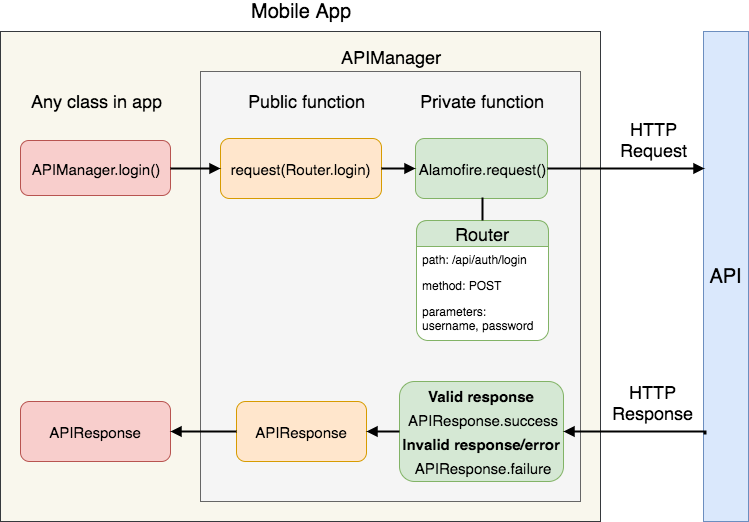
\includegraphics[width=\textwidth]{api-communication}
  \caption{The path of method calls and callbacks used when making a network request within the mobile app, namely logging the user in. The top row of arrows represent method calls being made from the app whilst the bottom row of arrows represent the callbacks for each method once the network response is received.}
  \label{fig:api-communication}
\end{figure}

\subsection{Tracking and saving walks}

Implementing the walk tracking component of the app was a main part of the project and the foundation that other parts of the app could be built upon. As was designed, when the user chooses to start tracking a walk a map is displayed showing the route from the user's location and statistics about the walk currently being tracked.

A location manager, part of the Core Location framework of the iOS SDK, was used to determine the geographical location of a user. The class to implement this is \verb|CLLocationManager|, which requests permission to use location services when the user's first opens the app. The integration of the Core Location framework in iOS means that the user's location obtained through the location manager can be displayed on an \verb|MKMapView| by simply setting its boolean instance variable \verb|showsUserLocation| to true.

\verb|CLLocationManager| has a delegate method \verb|didUpdateLocations()| that is automatically called by the operating system every time new location data from the user is available. This method passes in an array of \verb|CLLocation| as a parameter, the class which represents the location data generated by a location manager. A \verb|CLLocation| object stores the coordinate of a location by its latitude and longitude, and other details such as the altitude and accuracy. When this delegate method is called, the locations array parameter is appended to class variable \verb|locations| to record a history of a walk.

The distance of a walk, stored as a floating point variable in the class, is also calculated and updated in \verb|didUpdateLocations()|. \verb|CLLocation| provides an instance method to return the distance in metres between the receiver's location and another location. For each new location that is passed into the \verb|didUpdateLocations()| method, the distance is calculated between that location and the last location in the global locations array, which is then added to the global distance variable. This global distance variable therefore keeps track of the distance between all of the locations in the global locations array.

With the route of the walk and its distance now being logged, the UI had to be updated to display this information. To display the statistics about a walk, a timer was employed that fired every second. The duration of a walk was stored in seconds in a global class integer variable. Each second when the timer fired, this global time variable is incremented by one to track the duration of the walk. The time and distance variables are then formatted and displayed on the screen.

To display the walk route as a line on the map, I had to use the \verb|MKPolyline| class in the MapKit framework. An \verb|MKPolyline| is a shape that can be constructed via one or more coordinates. In \verb|didUpdateLocations()|, a polyline is constructed between the last coordinate in the global locations array and each location from the list of new locations parameter. This polyline is then added to the map by using the \verb|MKMapView| \verb|add()| instance method. An \verb|MKMapView| delegate method was also used to adjust the colour and thickness of the line drawn on the map.

% maybe move this to separate subsection

Once the user chooses to end their current walk, they are presented with an option to save the walk to their profile. A popup appears prompting the user to enter a name for the walk, which is used to identify the walk on the user's profile. After a name has been entered, a \verb|POST /walks/create/| request is sent to the API to store the walk in the database. This request accepts a number of fields to define the walk as parameters in the request body. The map route, implemented by the array of \verb|CLLocation| mentioned previously, is sent in the request as a JSON string representing an array of arrays of floating point numbers, with each array element corresponding to a coordinate in the form of longitude and latitude, like so:

\begin{center}
  \verb|[-0.174877, 51.498800], [-0.174523, 51.497810]]|
\end{center}

This JSON string is then parsed by the API and stored in the database using the GeoJSON format ***ref***, a specially designed format used to encode geographical data structures. An array of coordinates used in this project can be formatted in GeoJSON using the \verb|MultiPoint| geometry type.

\subsection{Displaying points of interest on a map}

In order for the data about the plaques to be retrieved, another Router had to be defined in the mobile app. Two endpoints were required for this router: one to gather a list of plaques inside a given coordinate region, and another to request detailed information about a plaque given its ID.

The OpenPlaques API is able to return data in a number of formats including JSON, which made it easy to parse responses since JSON had already been used previously in network calls. An area can be queried in OpenPlaques to find what plaques are present by specifying the top-left and bottom-right coordinates of the area's bounding box. The JSON returned is a list of details about the plaques, with each element containing the plaque's unique ID, coordinates and inscription.

% add example bounding box API request and the map region it would query

To display the plaque data on a map during a walk, repeated requests were made to the OpenPlaques API while the user was walking. A request is made every 60 seconds to search for plaques in an area of 500 metres squared with the centre at the user's location. The time interval and area span values were chosen to reduce the number of requests made to the API and also to ensure that the user could not walk into a new area before the new area request had been made.

An array of Plaque structs was used to store the data retrieved from the bounding box API request. While not all data is returned from said request, the coordinates enabled me to display all of the plaques as pins on the map by creating a subclass of \verb|MapKit|'s \verb|MKPointAnnotation| class for each plaque and calling the \verb|MKMapView| instance method \verb|addAnnotation()|.

% talk about removing old pins and not adding duplicates

\subsection{Gamification} \label{subsection:gamification}
% should this be in mobile app section?
% do I even need mobile app section?

The structure of the points system first needed to be implemented in the API, which the mobile app could then conform to. An object was defined as an enumeration in the back-end to represent the possible achievement types that could be gained from tracking a walk. Upon creating a walk via the \texttt{POST /walks/create} endpoint, the achievements parameter is checked against the list of valid achievement types. If one of the achievements is not valid, a \textbf{400 Bad Request} error is returned to the client.

% structure of achievements parameter

In the mobile app, a similar enumeration is defined to match the valid achievements listed in the back-end. When the user is saving a walk, the app checks whether there are achievements that the user should earn for the walk currently being saved. The achievements are sent to the server in the form of an array of dictionaries -- each element in the array a valid achievement with dictionary keys \textit{name} and \textit{value}, referring to the achievement type and number of points scored respectively. An example of a list of achievements sent in a request is as follows:

\begin{center}
  \verb|[{"name":"DAY_STREAK","value":4},{"name":"DISTANCE","value":100}]|
\end{center}


\subsection{Inviting users to go on a walk}

% fairly basic implementation due to time constraints
% would've liked to do more like live walk tracking, which is discussed in future extensions

As with other features of the project, the back-end implementation was completed first. For walk invitations, four endpoints had to be created:

\begin{itemize}
  \item \verb|POST /users/invite| creates a new Invite document in the database with the sender as the user sending the request (verified by the JWT) and the recipients specified as a parameter in the request body. It also sends a push notification to recipients' iOS devices if possible.

  \item \verb|GET /invites/:inviteID/accept| marks the invite with the specified invite ID as accepted for that user, given that the user has permission (if the invite was sent to them).

  \item \verb|GET /invites/:inviteID/decline| declines the specified invite given the user has permission, deleting the invite document from the database.

  \item \verb|GET /invites/:inviteID/start_walk| notifies the API that the sender has started the walk for a given invite. Due to time constraints, the current implementation simply deletes the invitation from the database so that it does not remain in the list of a user's received invites, however in the future I would like to implement a live tracking system as discussed in Section ***.
\end{itemize}

In the mobile app, the invites tab was implemented using a table view and a segmented control as designed in Section \ref{subsection:user-interface}. Depending on the selected segment in the segmented control, the table view was used to display either the user's sent or received invites. When the user select a different segment, a delegate method is called that pulls any new data from the API and refreshes the table view to display the correct data corresponding to the segment.

Custom table view cell classes were created to display both the sent and received invites, containing custom views and buttons depending on the invite type. The common attributes between the cells, such as the invite name and date, were collected into a superclass that both the sent and received invite cells conformed to. The two types of cells can be seen in Figure ***.

% add image of sent and received table view cells

\section{Challenges}


